\documentclass[11pt,english]{article}

%%%%%%%%%%%%%%%%%%%%%%%%%%%%%%%%%%%%%%%%%%%%%%%%%%%%%%%%%%%
% Packages
%%%%%%%%%%%%%%%%%%%%%%%%%%%%%%%%%%%%%%%%%%%%%%%%%%%%%%%%%%%

% Package imports are stored in /assets/base-packages.tex
% Packages specific to this pset can be imported here.

\listfiles
% paper size & margins
\usepackage{fullpage}
\usepackage[showframe=false,margin=1in]{geometry}
\parindent=0pt

% font management
\usepackage{relsize}
\usepackage[T1]{fontenc} % for properly hyphenating words with accented chars
\usepackage[latin1]{inputenc}
\usepackage{babel}

% figure management
\usepackage{epsfig}
\usepackage{graphicx}
\usepackage{wrapfig}
\usepackage{subfig}
%\usepackage{subfigure}
\usepackage[belowskip=0pt,aboveskip=0pt,font=small]{caption}
%\usepackage{subcaption}
\setlength{\intextsep}{7pt plus 0pt minus 0pt}

% math
\usepackage{amsmath, amsthm, amssymb}
%\usepackage{amstext}
\usepackage{textcomp}
\usepackage{stmaryrd}
\usepackage{upgreek}
\usepackage{bm}
\usepackage{cases}
\usepackage{mathtools}

% assorted
\usepackage{url}
\usepackage{breakurl}
\usepackage[colorlinks=true]{hyperref}
\usepackage{xspace}
\usepackage{comment}
\usepackage{color}
\usepackage{afterpage}
\usepackage[normalem]{ulem}
\usepackage{enumitem}



%%%%%%%%%%%%%%%%%%%%%%%%%%%%%%%%%%%%%%%%%%%%%%%%%%%%%%%%%%%
% Shortcuts
%%%%%%%%%%%%%%%%%%%%%%%%%%%%%%%%%%%%%%%%%%%%%%%%%%%%%%%%%%%
\usepackage{assets/mysymbols}
%%% load AMS-Latex Package
\usepackage{amsmath,amsfonts}
\usepackage{amsthm,amssymb,amsopn}
\usepackage{bm} % bold symbol
\usepackage{bbm}

% define fonts
\newcommand{\vct}[1]{\boldsymbol{#1}} % vector
\newcommand{\mat}[1]{\boldsymbol{#1}} % matrix

%%%% Special math symbols
\newcommand{\field}[1]{\mathbb{#1}}
\newcommand{\R}{\field{R}} % real domain
\newcommand{\C}{\field{C}} % complex domain
\newcommand{\F}{\field{F}} % functional domain
%\newcommand{\T}{^{\top}\!\!} % transpose
\newcommand{\T}{^{\textrm T}} % transpose
\newcommand{\TN}{^{-\textrm T}} % transpose
\newcommand{\Lagr}{\mathcal{L}}


%%% define constant
\newcommand{\cst}[1]{\mathsf{#1}}

%% operator in linear algebra, functional analysis
\newcommand{\inner}[2]{#1\cdot #2}
%\newcommand{\norm}[1]{\|#1\|}
\newcommand{\twonorm}[1]{\|#1\|_2^2}
% operator in functios, maps such as M: domain1 --> domain 2
\newcommand{\Map}[1]{\mathcal{#1}}

% operator in probability: expectation, covariance,
\newcommand{\ProbOpr}[1]{\mathbb{#1}}
% independence
\newcommand\independent{\protect\mathpalette{\protect\independenT}{\perp}}
\def\independenT#1#2{\mathrel{\rlap{$#1#2$}\mkern2mu{#1#2}}}
% conditional independence
\newcommand{\cind}[3]{{#1} \independent{#2}\,|\,#3}
% conditional expectation
\newcommand{\cndexp}[2]{\ProbOpr{E}\,[ #1\,|\,#2\,]}

% operator in optimization
%\DeclareMathOperator{\argmax}{arg\,max}
%\DeclareMathOperator{\argmin}{arg\,min}
%\newcommand{\todo}[1]{{\color{red}#1}}


% environment
\newtheorem{thm}{Theorem}

\newcommand{\eat}[1]{}

\newcommand{\hide}[1]{}
%\newcommand{\solution}{{\Large \vspace{5mm} \textbf{{\color{red}Solution:}}\newline\newline}}

\newcommand{\diff}{\mathop{}\!\mathrm{d}}
\newcommand{\Vop}{\textrm{T}}
\newcommand{\norminf}[1]{\norm{#1}_\infty}

% definitions for PS4
\newcommand{\vecy}{\ensuremath{\mathbf{y}}\xspace}
\newcommand{\vecx}{\ensuremath{\mathbf{x}}\xspace}
\renewcommand{\argmax}{\operatornamewithlimits{argmax}}
\newcommand{\startsym}{\mbox{\scriptsize \texttt{<s>}}\xspace}
\newcommand{\stopsym}{\mbox{\scriptsize \texttt{</s>}}\xspace}
\newcommand{\best}{\ensuremath{\mathit{best}}\xspace}
\newcommand{\bestuptoi}{\ensuremath{\texttt{best}_{\leq i}}\xspace}
\newcommand{\bestuptot}{\ensuremath{\texttt{best}_{\leq t}}\xspace}
\newcommand{\completed}{\ensuremath{\texttt{comp}}\xspace}
\newcommand{\toptop}{\operatornamewithlimits{\mathbf{top}}}
\newcommand{\tuple}[1]{\ensuremath{\langle {#1} \rangle}}
\newcommand{\xuptot}{\ensuremath{\mathit{x}_{\leq t}}\xspace}


\renewcommand{\hide}[1]{}

%%%%%%%%%%%%%%%%%%%%%%%%%%%%%%%%%%%%%%%%%%%%%%%%%%%%%%%%%%%
% Title / Author
%%%%%%%%%%%%%%%%%%%%%%%%%%%%%%%%%%%%%%%%%%%%%%%%%%%%%%%%%%%
\begin{document}
\title{CS 4644/7643: Deep Learning\\
Spring 2025 \\
Problem Set 2} 

% NOTE: Any changes to instructor, TAs, or piazza link should be done in the file below
\author{Instructor: Zsolt Kira \\
TAs: Wei Zhou, Aryan Sarswat, Woo Chul Shin, Elias Cho, \\Haotian Xue, Sri Siddarth Chakaravarthy Prakash, Neelabh Sinha, David He, \\ Sriharsha Kocherla, Pratham Mehta, Ayush Patel, Cari He\\
Discussions: \url{https://piazza.com/class/m5k29i4gzsf4ab/}}
\date{Deadline: 11:59pm February 17st, 2025}
\maketitle


\paragraph*{Instructions}
\begin{enumerate}
\item We will be using Gradescope to collect your assignments.  Please read the following instructions for submitting to Gradescope carefully!
     \begin{itemize}
          \item
               Please upload separate pdfs for \textbf{HW2 Theory} and \textbf{HW2 Report} sections on Gradescope. The instructions for the latter are included in the coding section of the assignment.  \textbf{When submitting to Gradescope, please make sure to mark the page(s) corresponding to each problem/sub-problem}.
          \item
               For the \textbf{HW2 Code Part 1 and Part 2} components on Gradescope, 
               please use the \texttt{collect\_submission.py} script provided and upload the resulting zip files to each Gradescope section respectively. Please make sure you have saved the most recent version of your code.
          \item
               Note: This is a large class and Gradescope's assignment segmentation features are essential.
               Failure to follow these instructions may result in parts of your assignment not being graded.
               We will not entertain regrading requests for failure to follow instructions.
     \end{itemize}

\item
     \LaTeX'd solutions are strongly encouraged (solution template available in the zip file in HW2 under the Assignments tab on Canvas),
     but scanned handwritten copies are acceptable.
     Hard copies are \textbf{not} accepted.


\item We generally encourage you to collaborate with other students.

You may talk to a friend, discuss the questions and potential directions for solving them. However, you need to write
your own solutions and code separately, and \emph{not} as a group activity.
Please list the students you collaborated with. \\ \\
\end{enumerate}
\newpage

%%%%%%%%%%%%%%%%%%%%%%%%%%%%%%%%%%%%%%%%%%%%%%%%%%%%%%%%%%%
% Body
%%%%%%%%%%%%%%%%%%%%%%%%%%%%%%%%%%%%%%%%%%%%%%%%%%%%%%%%%%%

\section{Collaborators [0.5 points]}

Please list your collaborators and assign this list to the corresponding section of the outline on Gradescope. If you don't have any collaborators, please write 'None' and assign it to the corresponding section of the Gradescope submission regardless.

% This is for next year (2026)
\section{Activation Function}
\begin{enumerate}[start]

\item
\textbf{[2 points]}

In neural networks, activation functions introduce non-linearities, enabling the network to approximate complex functions. One of the desirable properties for an activation function is to be \emph{zero-centered}. Being zero-centered helps in achieving faster convergence during training, as the weights can adjust in both positive and negative directions more efficiently. Additionally, zero-centered functions can help mitigate the vanishing gradient problem, ensuring that gradients during backpropagation do not diminish too quickly.

Definition: A function \( g(x) \) is said to be zero-centered if, for every value \( x \) in its domain where \( g(x) \) is positive, there exists an equivalent negative value \( -x \) such that:
\[
  g(-x) = -g(x).
\]
In other words, the function is symmetric about the origin, producing positive outputs for positive inputs and negative outputs for negative inputs.

Consider the following activation function, defined for all real \(x\):
\[
  g(x) \;=\; \frac{x}{1 + |x|}.
\]

\begin{enumerate}
  \item Zero-Centered Property.
  Show that \( g(x) \) is zero-centered by proving \( g(-x) = -g(x) \) for all \( x \). 
  (Hint: carefully handle the absolute value.)

  \item Derivative and Gradient Behavior
    \begin{enumerate}
      \item Compute the derivative \( g'(x) \) for \( x \neq 0 \).
      \item Evaluate \( g'(0) \) (Hint: the function is continuous).
      \item Based on your results, show whether \( g(x) \) might cause vanishing or exploding gradients for large values of \( |x| \) (Hint: show the limits).
    \end{enumerate}
\end{enumerate}

\end{enumerate}

\section{Gradient Descent}
\begin{enumerate}[start]

\item
\textbf{[3 points]}

We often use iterative optimization algorithms such as Gradient Descent to
find $\mathbf{w}$ that minimizes a loss function $f(\mathbf{w})$. Recall that in gradient descent,
we start with an initial value of $\mathbf{w}$ (say $\mathbf{w}^{(1)}$) and iteratively take a step in the direction
of the negative of the gradient of the objective function \ie
%
\begin{equation}
\mathbf{w}^{(t+1)} = \mathbf{w}^{(t)} - \eta\nabla f(\mathbf{w}^{(t)})
\end{equation}
%
for learning rate $\eta > 0$.

In this question, we will develop a slightly deeper understanding of this update rule, in particular for 
minimizing a convex function $f(\mathbf{w})$. Note: this analysis will not directly carry over to training neural networks 
since loss functions for training neural networks are typically not convex, but this will (a) develop intuition 
and (b) provide a starting point for research in non-convex optimization (which is beyond the scope of this class). 


Recall the first-order Taylor approximation of $f$ at $\mathbf{w}^{(t)}$:
%
\begin{align}\label{first-order-approx}
f(\mathbf{w}) \approx f(\mathbf{w}^{(t)}) + \langle \mathbf{w}-\mathbf{w}^{(t)},
\nabla f(\mathbf{w}^{(t)}) \rangle
\end{align}
%
When $f$ is convex, this approximation forms a lower bound of $f$, \ie 
\begin{align}
f(\mathbf{w}) \ge 
\underbrace{
f(\mathbf{w}^{(t)}) + \langle \mathbf{w}-\mathbf{w}^{(t)}, 
\nabla f(\mathbf{w}^{(t)}) \rangle
}_{\text{affine lower bound to $f(\cdot)$}}
 \quad \forall \mathbf{w}
\end{align}
%

Since this approximation
is a `simpler' function than $f(\cdot)$, we could consider minimizing the approximation instead of $f(\cdot)$.
Two immediate problems: (1) the approximation is affine (thus unbounded from below) and
(2) the approximation is faithful for $\mathbf{w}$ close to $\mathbf{w}^{(t)}$.
To solve both problems, we add a squared $\ell_2$ \emph{proximity term} to the approximation minimization:
%
\begin{equation}
\argmin_\mathbf{w}
\underbrace{
f(\mathbf{w}^{(t)}) + \langle \mathbf{w}-\mathbf{w}^{(t)}, \nabla f(\mathbf{w}^{(t)}) \rangle
}_{\text{affine lower bound to $f(\cdot)$}}
+
\underbrace{
\frac{\lambda}{2}
}_{\text{trade-off}}
\underbrace{
\norm{\mathbf{w} - \mathbf{w}^{(t)}}^2
}_{\text{proximity term}}
\end{equation}
%

Notice that the optimization problem above is an unconstrained quadratic programming problem,
meaning that it can be solved in closed form (hint: gradients).

What is the solution $\mathbf{w}^*$ of the above optimization?
What does that tell you about the gradient descent update rule?
What is the relationship between $\lambda$ and $\eta$?


\item
\textbf{[Extra Credit - 2 points]}

Let's prove a lemma that will initially seem devoid of the rest of the analysis but will come 
in handy in the next sub-question when we start combining things. 
Specifically, the analysis in this sub-question holds for any $\mathbf{w}^{\star}$, but in the next sub-question  
we will use it for $\mathbf{w}^{\star}$ that minimizes $f(\mathbf{w})$. 

Consider a sequence of vectors $\mathbf{v}_1, \mathbf{v}_2, ..., \mathbf{v}_T$, 
and an update equation of the form $\mathbf{w}^{(t+1)} = \mathbf{w}^{(t)} - \eta\mathbf{v}_{t}$ 
with $\mathbf{w}^{(1)} = 0$. 
Show that: 

\begin{equation}
\sum_{t=1}^T \langle \mathbf{w}^{(t)}-\mathbf{w}^{\star}, \mathbf{v}_t \rangle \leq
\frac{\norm{\mathbf{w}^{\star}}^2}{2\eta} + \frac{\eta}{2} \sum_{t=1}^T \norm{\mathbf{v}_t}^2
\end{equation}

\item
\textbf{[Extra Credit - 2 points]}

Now let's start putting things together and analyze the convergence rate of gradient descent \ie
how fast it converges to $\mathbf{w}^\star$. For this question, assume that $f$ is convex and $\rho$-Lipschitz. A function that is $\rho$-Lipschitz is one where the norm of its gradient is bounded by $\rho$, i.e. $\norm{\nabla f(\mathbf{w})} \leq \rho$.

First, show that for $\mathbf{\bar w} = \frac{1}{T} \sum_{t=1}^T \mathbf{w}^{(t)}$

\begin{equation}
f(\mathbf{\bar w}) - f(\mathbf{w}^\star) \leq \frac{1}{T} \sum_{t=1}^T
\langle \mathbf{w}^{(t)}-\mathbf{w}^{\star}, \nabla f(\mathbf{w}^{(t)}) \rangle
\end{equation}

Next, use the result from part $2$, with upper bounds $B$ and $\rho$ for
$\norm{\mathbf{w}^\star}$ and $\norm{\nabla f(\mathbf{w}^{(t)})}$
respectively and show that for fixed $\eta = \sqrt{\frac{B^2}{\rho^2T}}$,
the convergence rate of gradient descent is $\mathcal{O}(1/\sqrt{T})$
\ie the upper bound for $f(\mathbf{\bar w}) - f(\mathbf{w}^\star)$
$\propto$ $\frac{1}{\sqrt{T}}$.

\end{enumerate}


\section{Automatic Differentiation}
\begin{enumerate}[resume]

\item
\textbf{[4 points]}

In practice, writing the closed-form expression of the derivative of
a loss function $f$ w.r.t. the parameters of a deep neural network is hard
(and mostly unnecessary) as $f$ becomes complex. Instead, we define
computation graphs and use the automatic differentiation algorithms (typically backpropagation) to compute
gradients using the chain rule. For example, consider the expression

\begin{equation}
f(x, y) = (x+y)(y+1)
\end{equation}

Let's define intermediate variables $a$ and $b$ such that

\begin{equation}
a = x + y
\end{equation}
%
\begin{equation}
b = y + 1
\end{equation}
%
\begin{equation}
f = a \times b
\end{equation}
A computation graph for the ``forward pass'' through $f$ is shown in \figref{fig:graph}. 

\begin{figure}[h]
  \centering
    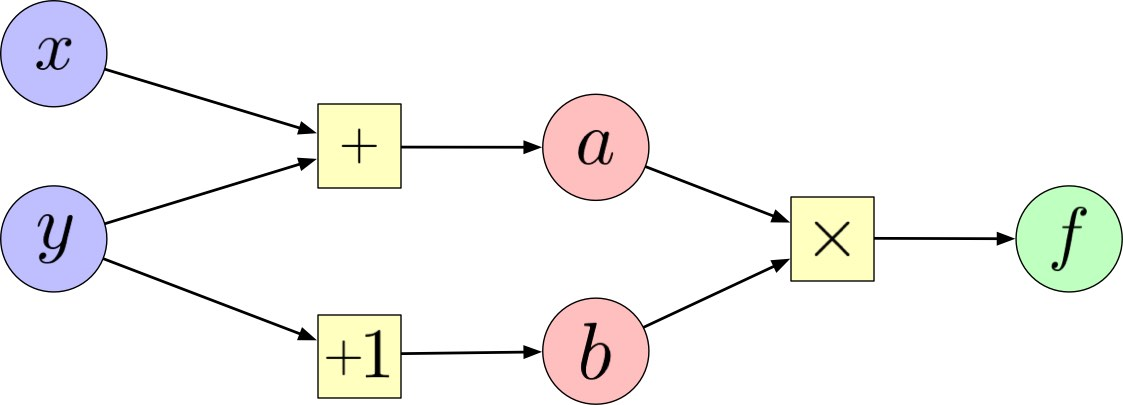
\includegraphics[width=0.5\textwidth]{assets/comp_graph_example.jpg}
    \caption{}
    \label{fig:graph}
\end{figure}

We can then work backwards and compute the derivative of $f$ w.r.t. each
intermediate variable ($\frac{\del f}{\del a}$, $\frac{\del f}{\del b}$) and
chain them together to get $\frac{\del f}{\del x}$ and $\frac{\del f}{\del y}$. \\

Let $\sigma(\cdot)$ denote the standard sigmoid function. Now, for the following vector function:

\begin{align}
f_1(w_1, w_2) &= \cos(w_1)\cos(w_2) + \sigma(w_2) \\
f_2(w_1, w_2) &= ln(w_1 + w_2) + w_1^2 w_2
\end{align}

\begin{enumerate}
\item Draw the computation graph (you might find \href{https://draw.io/}{draw.io} useful for this). Compute the value of $f$ at $\vec{w} = (1, 2)$.
\item At this $\vec{w}$, compute the Jacobian $\frac{\del \vec{f}} {\del \vec{w}}$ using numerical differentiation (using $\Delta w$ = 0.01).
\item At this $\vec{w}$, compute the Jacobian using forward mode auto-differentiation.
\item At this $\vec{w}$, compute the Jacobian using backward mode auto-differentiation.
\item Don't you love that software exists to do this for us?
% making use of intermediate variables and reusing
%nodes (caching results) where necessary. Then apply the chain rule and compute
%$\frac{\del f}{\del w}$.
\end{enumerate}

\end{enumerate}

\section{Convolutions}
\begin{enumerate}[resume]

\item 
\textbf{[5 points]}

We'll start to introduce the properties of convolutions here that serve as a foundation for many computer vision applications in deep learning. 
In class, we discussed convolutions. In this question, we will develop formal intuition around a slight modification of that idea -- circular convolutions. 


First, let's define a circular convolution of two n-dimensional vectors $\mathbf{x}$ and $\mathbf{w}$:

\begin{equation}
(\mathbf{x} * \mathbf{w})_{i} = \sum_{k=0}^{n-1} x_{k} w_{(i-k)\text{ mod } n}  
\end{equation}

We can write the above equation as a matrix-vector multiplication. 

Given an n-dimensional vector $\mathbf{a} = (a_0, ..., a_{n-1})$, we define the associated matrix $C_\mathbf{a}$ whose first column is made up of these numbers, and each subsequent column is obtained by a circular shift of the previous column. 

\[ C_\mathbf{{a}} = 
\begin{bmatrix}
    a_0 & a_{n-1} & a_{n-2} & \dots  & a_1 \\
    a_1 & a_0 & a_{n-1} & & a_2  \\
    a_2 & a_1 & a_0 &  & a_3\\
    \vdots &  & \ddots  & \ddots & \vdots\\
    a_{n-1} & a_{n-2} & a_{n-3} & \dots & a_0 \\
\end{bmatrix}
\]


Such matrices are called \textit{circulants}. Any convolution $\mathbf{x} * \mathbf{w}$ can be equivalently represented as a multiplication by the circulant matrix $C_\mathbf{a}\mathbf{x}$.


Note that a circulant matrix is a kind of Toeplitz matrix with the additional property that $a_i=a_{i+n}$. 
Next, let's introduce a special type of circulant called a shift matrix. A shift matrix is a circulant matrix where only one dimension of the vector $\mathbf{a}$ can be set to 1, \textit{i.e.}, $\mathbf{a} = (0, 1, ..., 0)$. Let $S$  be the circular right-shift operator,
defined by the following action on vectors:

\[ S\mathbf{x} = 
\begin{bmatrix}
    0 &  &  &  & 1 \\
    1 &  &  & & \\
    &  & \ddots & \ddots & \\
    &  &  & 1 & 0 \\
\end{bmatrix}
\begin{bmatrix}
    x_0 \\
    x_1 \\
    \vdots \\
    x_{n-1}
\end{bmatrix}
=
\begin{bmatrix}
    x_{n-1} \\
    x_0 \\
    \vdots \\
    x_{n-2}
\end{bmatrix}
\]

Notice that after applying the shift-matrix, all the element of $\mathbf{x}$ have been shifted by 1.

\begin{enumerate}
\item Prove that \emph{any} circulant matrix is commutative with a shift matrix. 
Note that this directly implies that convolutions are commutative with shift operators. 
\end{enumerate}

This leads to very important property called translation or shift equivariance. A function is shift equivariant if $f(S\mathbf{x})=Sf(\mathbf{x}).$ Convolution's commutativity with shift implies that it does not matter whether we first shift a vector and then convolve it, or first convolve and then shift -- the result will be the same. 
Notice that you just proved that circular convolutions are shift equivariant. 

\begin{enumerate}[resume]
\item Now prove that the a (circular) convolution is the \emph{only} linear operation with shift equivariance. (Hint: how do you prove a bidirectional implication?)

\item (Open-ended question) What does this tell you about designing deep learning architectures for processing 
spatial or spatio-temporal data like images and videos? 
\end{enumerate}

\end{enumerate}


\section{SGD}
\begin{enumerate}[resume]

\item 
\textbf{[3 points]}

Consider an objective function comprised of $N=2$ terms:

\begin{equation}
f(w) = \frac{1}{2} (w-2)^2 + \frac{1}{2}(w+1)^2
\end{equation}

Now consider using SGD (with a batch-size $B=1$) to minimize this objective. Specifically, in each iteration,
we will pick one of the two terms (uniformly at random), and take a step in the direction of the negative gradient, with a constant
step-size of $\eta$.
%If we sample one data point every iteration,
%does SGD guarantee to decrease
You can assume $\eta$ is small enough that every update does result in improvement (aka descent) on the sampled term.

Is SGD guaranteed to decrease the overall loss function in every iteration? If yes, provide a proof. If no, provide a counter-example.

\end{enumerate}


\section{Paper Review}
\begin{enumerate}[resume]

\item 
\textbf{[4 points]}

The paper we will study in this homework is \textbf{`Understanding deep learning requires rethinking generalization'}, presented at the International Conference on Learning Representations (ICLR) in 2017.

The paper presents a set of interesting experiments and results to explore the phenomenon of generalization in deep neural networks, i.e, the difference in performance on the training and test sets, and the role of explicit and implicit regularization towards achieving this. The paper can be viewed \href{https://arxiv.org/abs/1611.03530}{here}.

Please discuss the following:
\begin{enumerate}
\item
Briefly summarize the key contributions, strengths and weaknesses of this paper.

\item
What is your personal takeaway from this paper? This could be expressed either in terms of relating the approaches adopted in this paper to your traditional understanding of learning parameterized models, or potential future directions of research in the area which the authors haven't addressed, or anything else that struck you as being noteworthy. 
\end{enumerate}

\textbf{Guidelines}: Please restrict your reviews to no more than 350 words (total length for answers to both the above questions).

\end{enumerate} 


\end{document}
